\PassOptionsToPackage{unicode}{hyperref}
\documentclass[aspectratio=1610, professionalfonts, 9pt]{beamer}

\usefonttheme[onlymath]{serif}
\usetheme[showtotalframes]{tudo}

\ifluatex
\usepackage{polyglossia}
\setmainlanguage{german}
\else
\ifxetex
\usepackage{polyglossia}
\setmainlanguage{german}
\else
\usepackage[german]{babel}
\fi
\fi


% Mathematik
\usepackage{amsmath}
\usepackage{amssymb}
\usepackage{mathtools}
\usepackage{cancel}
\usepackage{siunitx}

\usepackage{hyperref}
\usepackage{bookmark}

% Bibliographie 
\usepackage[
  backend=biber,   
  autolang=hyphen,
  citestyle=verbose, 
  giveninits=true,
]{biblatex}
\addbibresource{references.bib} 
\DefineBibliographyStrings{german}{andothers = {{et\,al\adddot}}}

% Tabellen
\usepackage{booktabs}

%%%%%%%%%%%%%%%%%%%%%%%%%%%%%%%%%%%%%%%%%%%%%%%%%%%%%%%%%%%%%%%%%%%%%%%%%%%%%%%%
%%%%%-------------Hier Titel/Autor/Grafik/Lehrstuhl eintragen--------------%%%%%
%%%%%%%%%%%%%%%%%%%%%%%%%%%%%%%%%%%%%%%%%%%%%%%%%%%%%%%%%%%%%%%%%%%%%%%%%%%%%%%%

%Titel:
\title{Gamma/Hadron-Seperation bei FACT}
%Autor
\author[M.~Sackel]{Maximilian Sackel}
%Lehrstuhl/Fakultät
\institute[Experimental Physics 5]{Experimental Physiks 5b \\  Astroteilchenphysik}
%Titelgrafik 
\titlegraphic{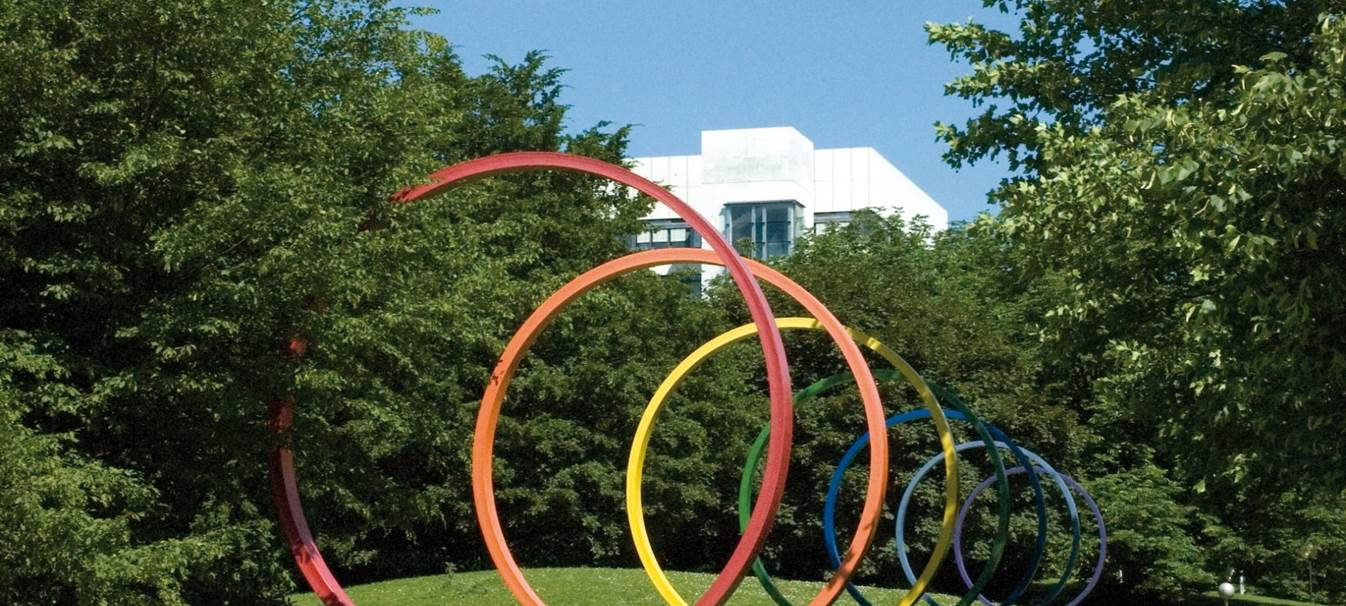
\includegraphics[width=0.7\textwidth]{images/tudo-title-2.jpg}}


\begin{document}

\maketitle

\section{Basics}
\begin{frame}
  \begin{figure}
	\centering
	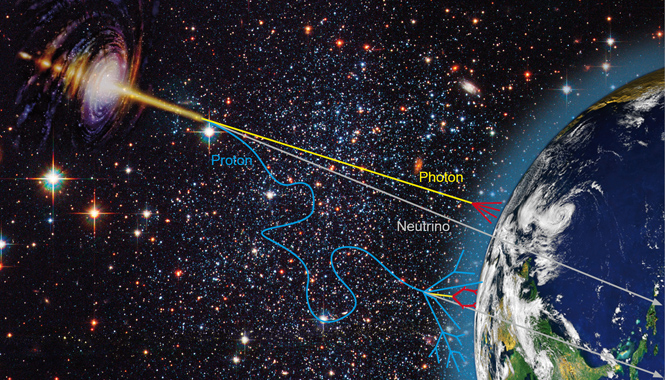
\includegraphics[width=0.8\textwidth]{./images/sources-detection.jpg} \\
	\caption{\cite{Overview}}
  \end{figure}
\end{frame}

\begin{frame}
  \begin{columns}
	\column{.3\textwidth}
	\begin{figure}
	  \centering
	  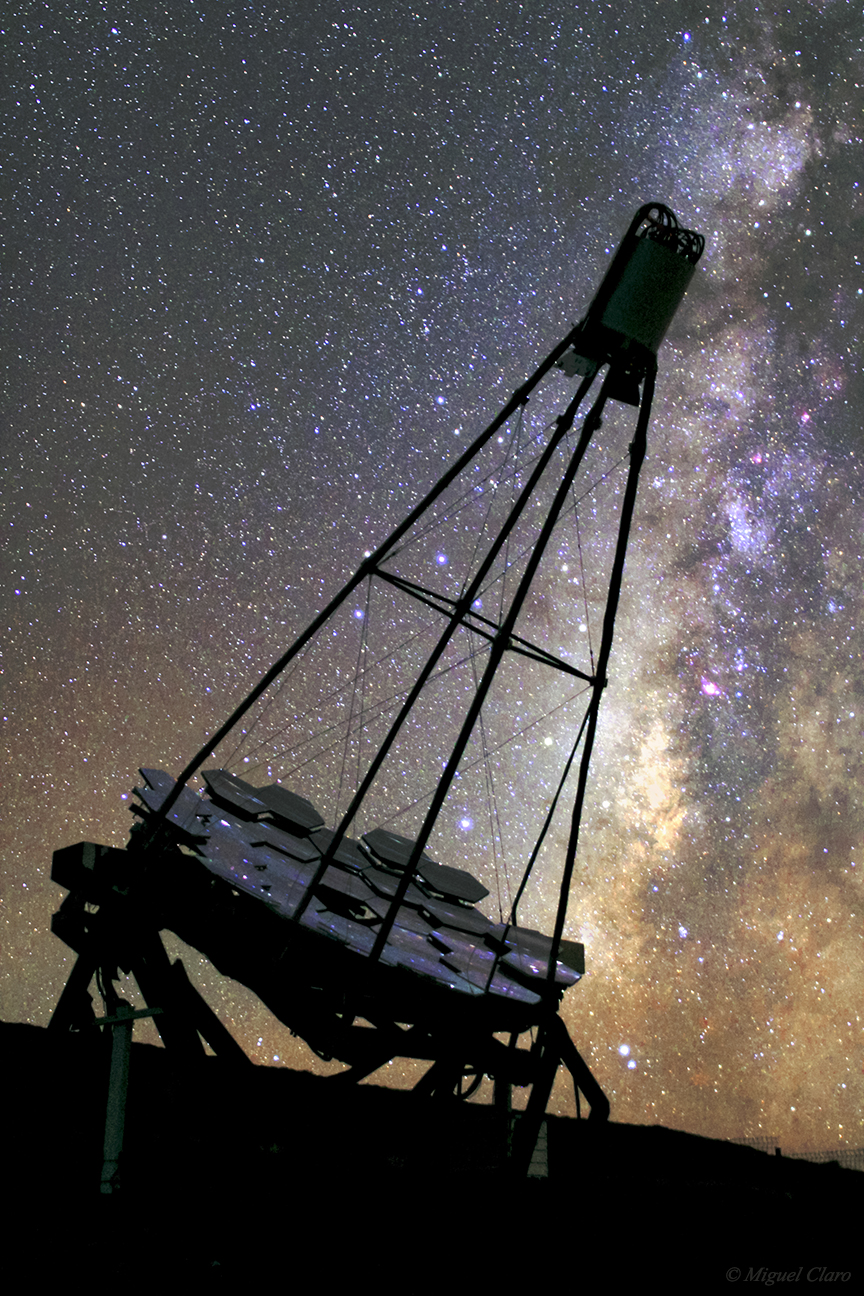
\includegraphics[height=0.8\textheight]{./images/FACT.jpg}
	  \caption{\cite{FACT}}
	\end{figure}
	\column{.7\textwidth}
	\only<1>{
	  \Huge
	  \centering
	  \textbf{F}irst G-\textbf{A}PD \textbf{C}herenkov \textbf{T}elescope
	}
	\only<2>{
	  \begin{figure}
		\centering
		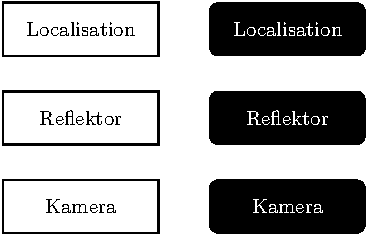
\includegraphics[height=0.8\textheight]{./tikz/FACT/FACT.pdf}
	  \end{figure}
	}
  \end{columns}
\end{frame}

\begin{frame}
  \begin{columns}
	\column{.2\textwidth}
	\begin{figure}
	  \centering
	  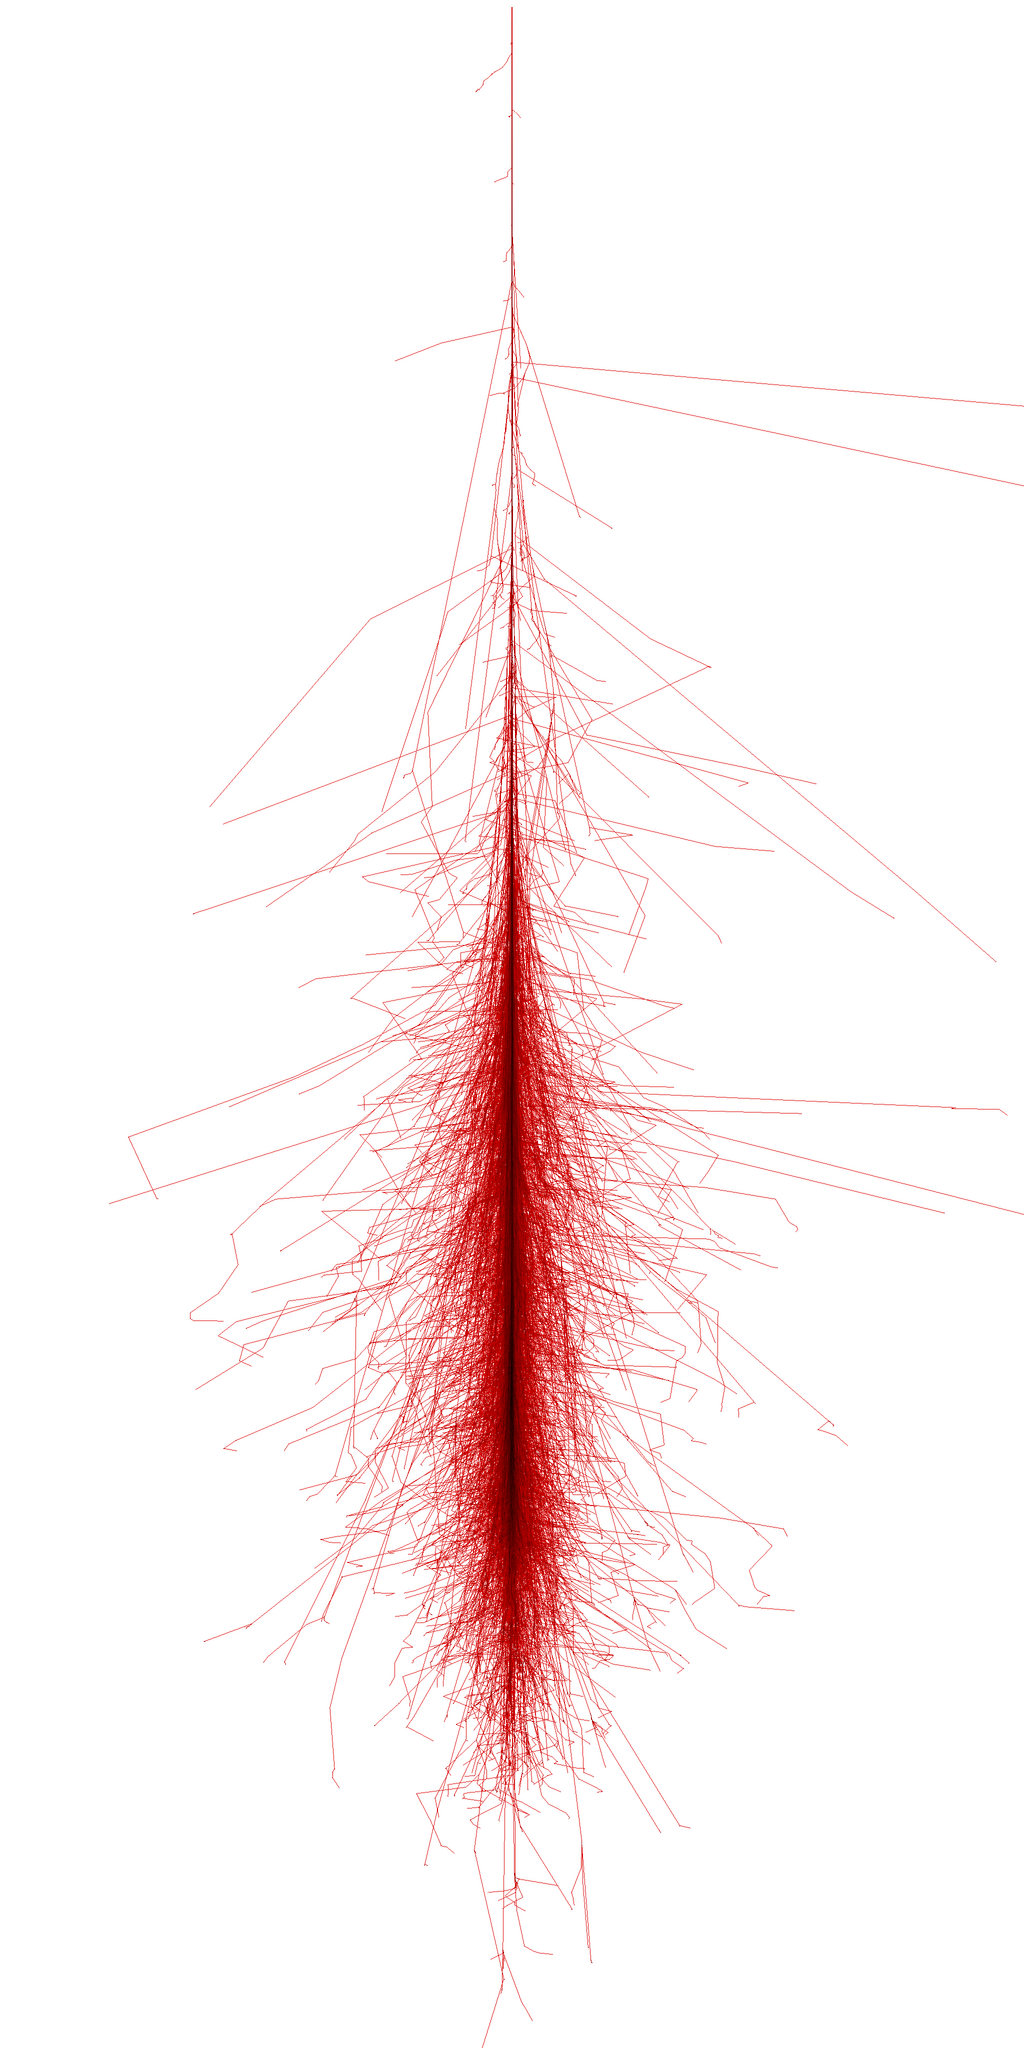
\includegraphics[width=\textwidth]{./images/photon_100GeV.png}
	  \caption{\cite{FACT}}
	\end{figure}
	\column{.3\textwidth}
	\begin{eqnarray*}
	  \gamma \rightarrow& e^{+} + e^{-} \\
	  e^{+} \rightarrow& e^{+'} + \gamma \\
	  e^{-} \rightarrow& e^{-'} + \gamma 
	\end{eqnarray*}
	\column{.2\textwidth}
	\begin{figure}
	  \centering
	  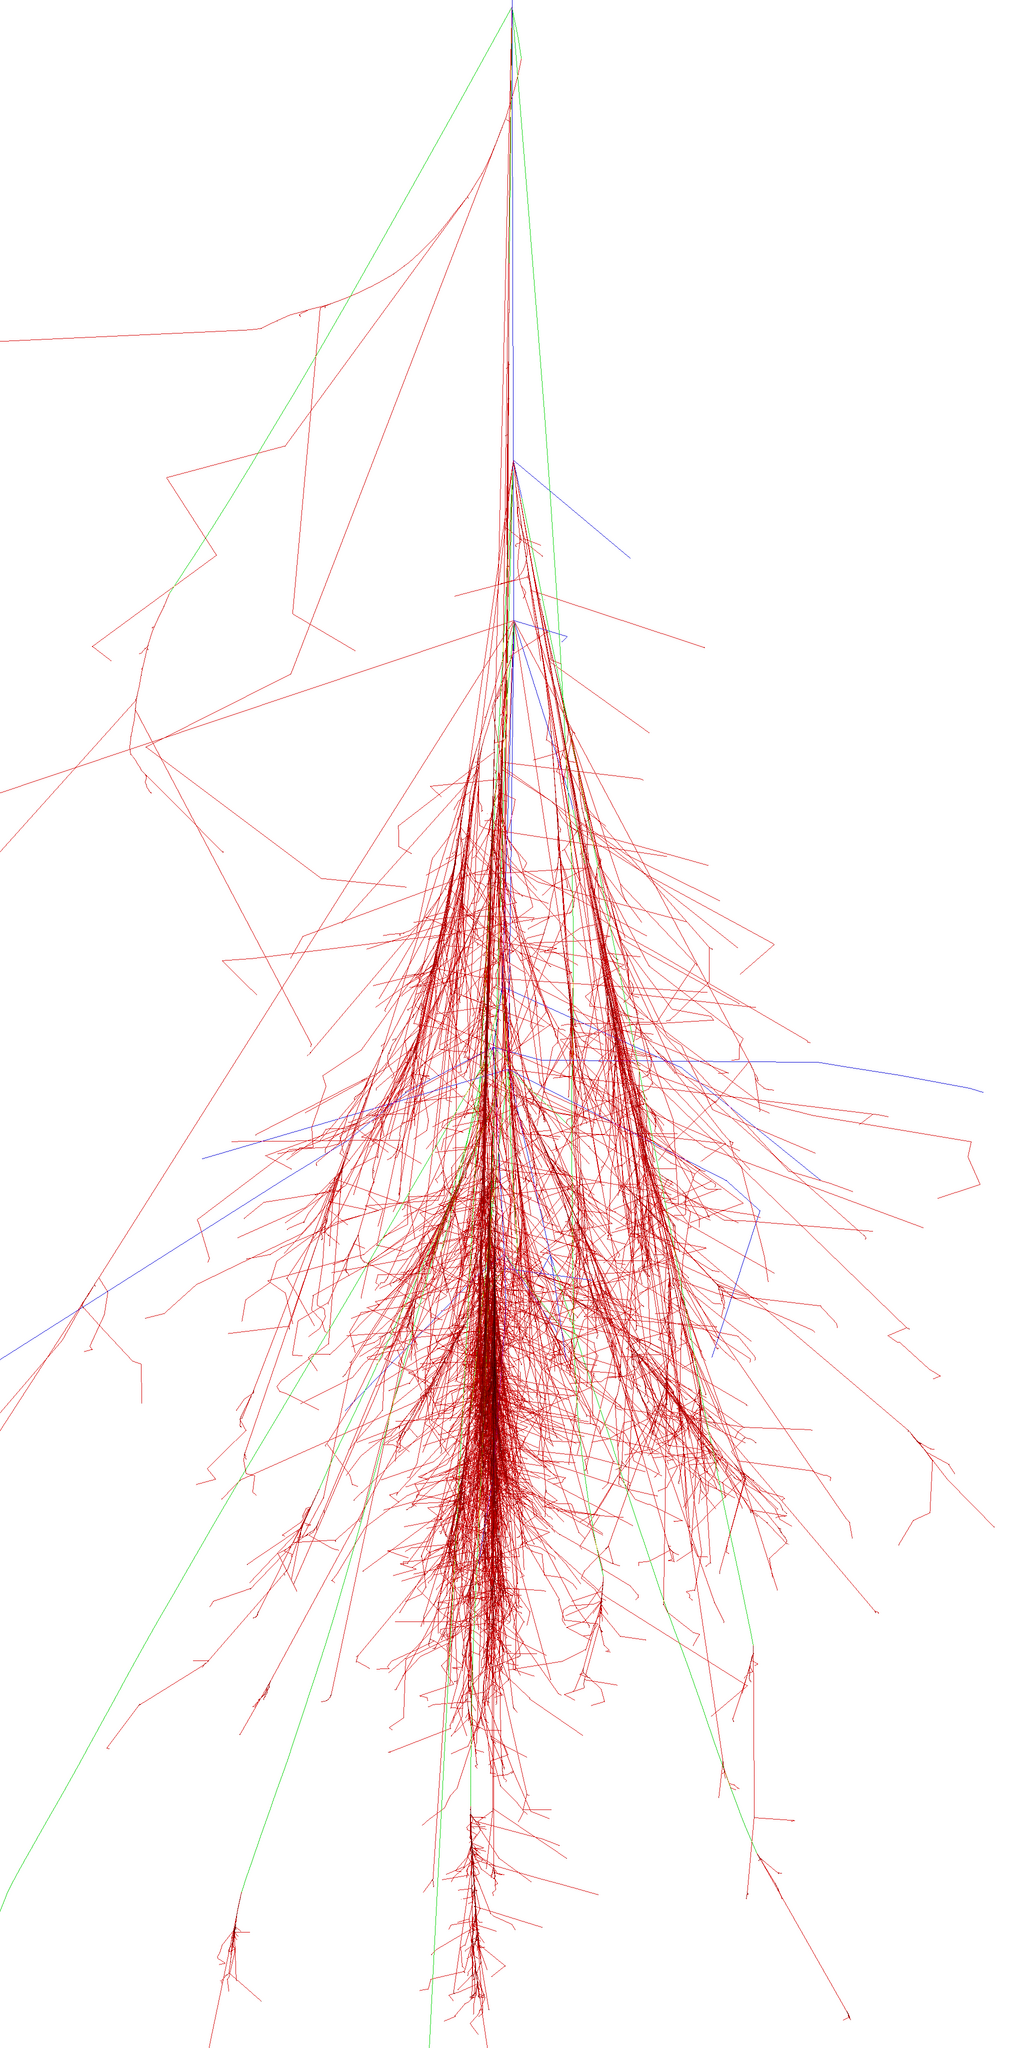
\includegraphics[width=\textwidth]{./images/proton_100GeV.png}
	  \caption{\cite{FACT}}
	\end{figure}
	\column{.3\textwidth}
	\begin{eqnarray*}
	  \pi^{0} \rightarrow& \gamma + \gamma \\
	  \pi^{+} \rightarrow& \mu^{+} + \nu_{\mu} \\
	  \pi^{-} \rightarrow& \mu^{-} + \bar{\nu}_{\mu}
	\end{eqnarray*}
  \end{columns}
\end{frame}

\begin{frame}
  \begin{columns}
	\column{.5\textwidth}
	\begin{figure}
	  \centering
	  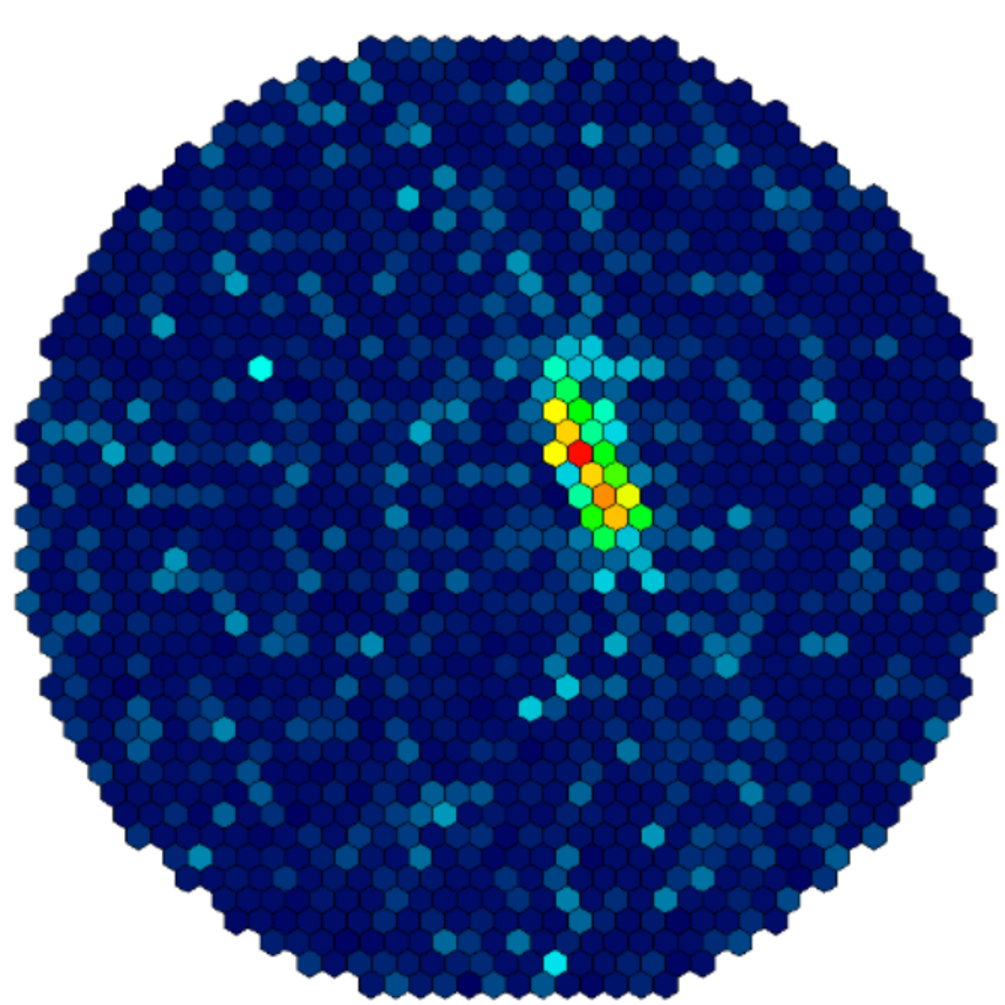
\includegraphics[height=0.8\textheight]{./images/Gamma.pdf}
	  \caption{\cite{FACT}}
	\end{figure}
	\column{.5\textwidth}
	\begin{figure}
	  \centering
	  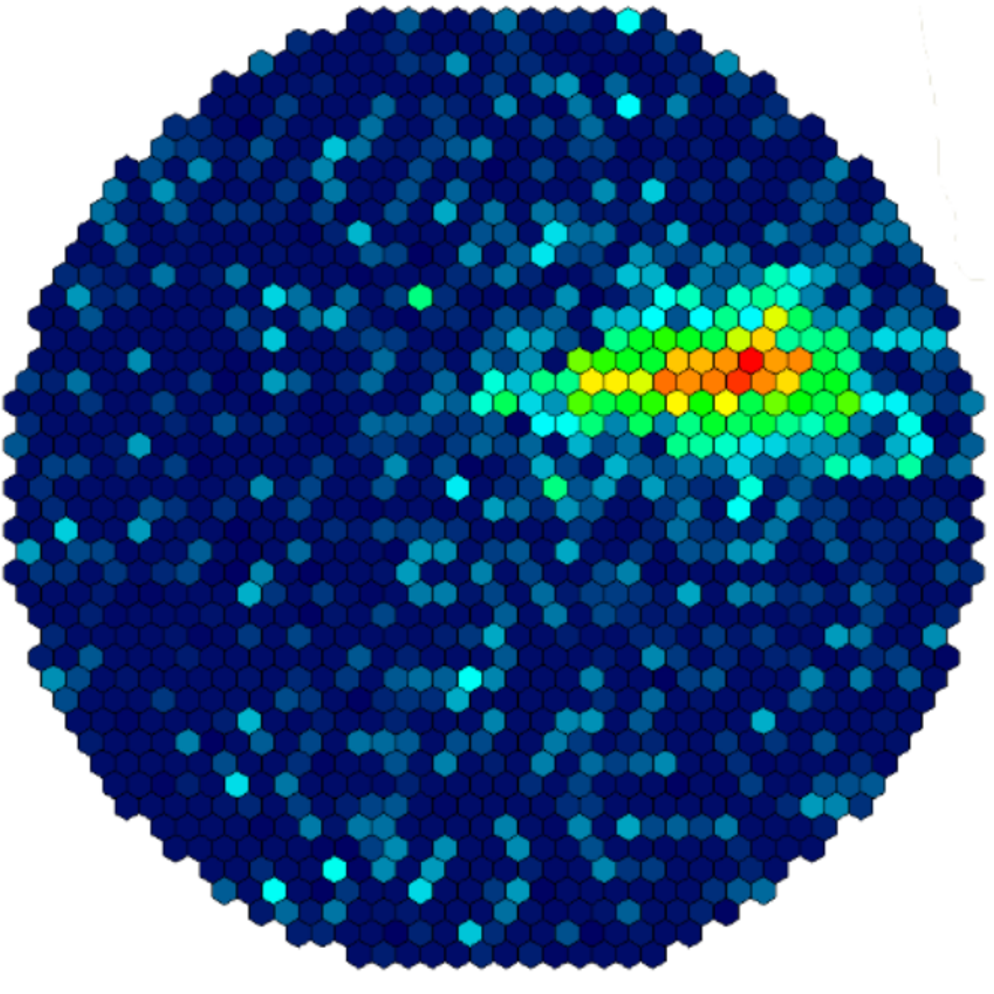
\includegraphics[height=0.8\textheight]{./images/Hadron.pdf}
	  \caption{\cite{FACT}}
	\end{figure}
  \end{columns}
\end{frame}


\begin{frame}
  \begin{columns}
	\column{.5\textwidth}
	\begin{figure}
	  \centering
	  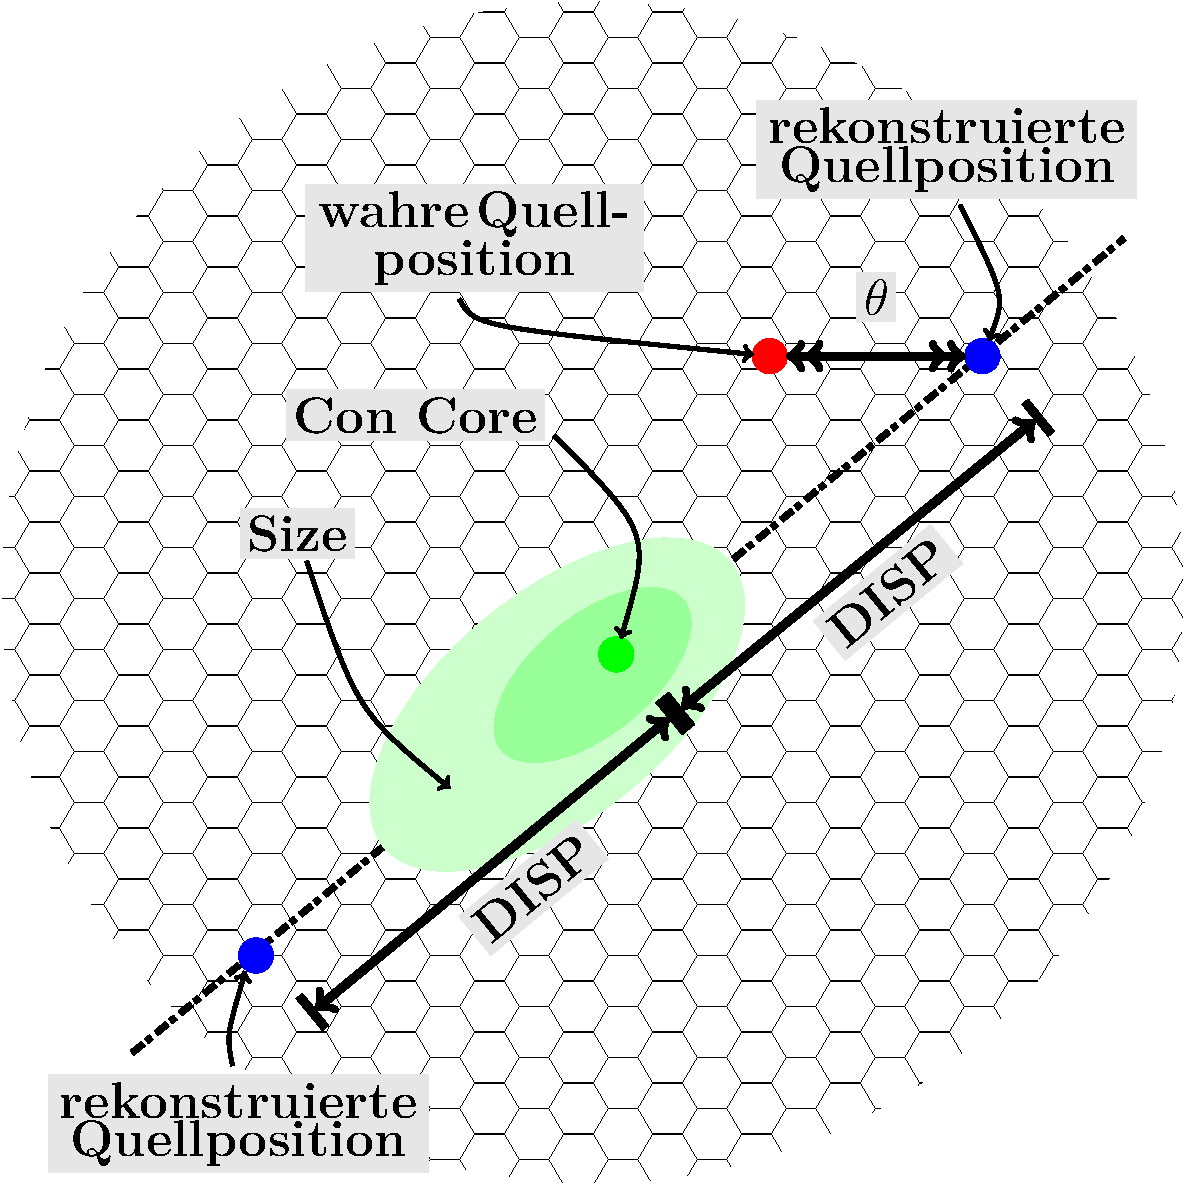
\includegraphics[height=0.8\textheight]{./images/camera.pdf}
	\end{figure}
	\column{.5\textwidth}
	\begin{itemize}
	  \item berechne Feature (Hillas Parameter) des Kamerabildes
	  \item Feature werden zum Klassifizieren benoetigt
	  \item Vorzeichen des Schauers nicht eindeutig
	\end{itemize}
  \end{columns}
\end{frame}

\begin{frame}
  \begin{columns}
	\column{.5\textwidth}
	\begin{figure}
	  \centering
	  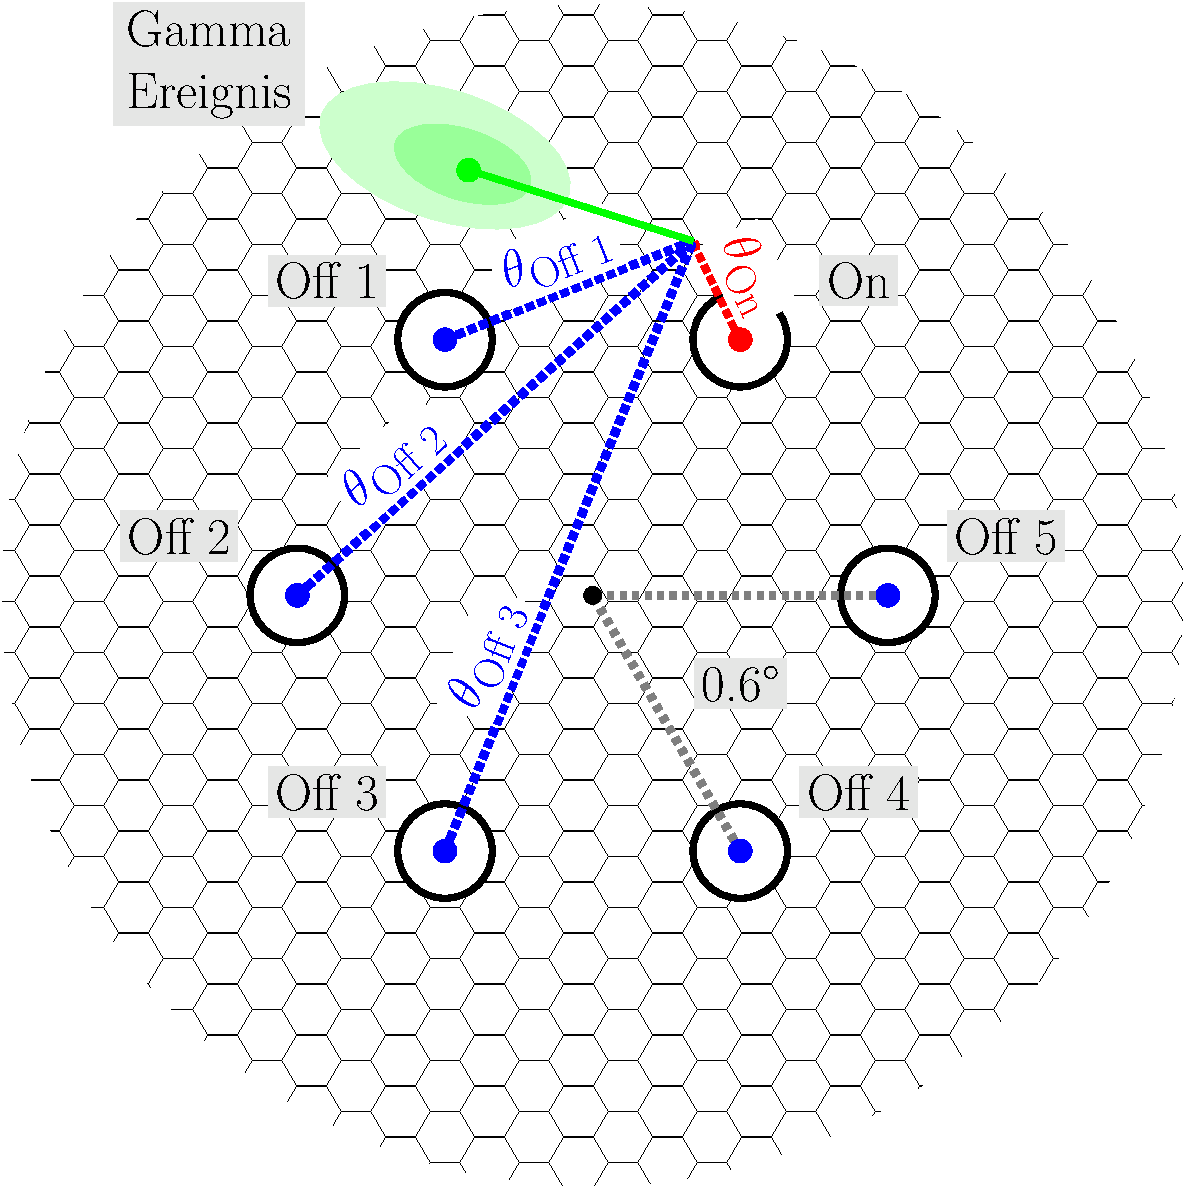
\includegraphics[height=0.8\textheight]{./images/wobble.pdf}
	\end{figure}
	\column{.5\textwidth}
	\begin{itemize}
	  \item FACT nimmt keine OFF-Daten
	  \item Daten werden im Wobble Modus genommen
	\end{itemize}
  \end{columns}
\end{frame}

\begin{frame}
  \begin{block}{Seperation}<1-2>
	\begin{figure}
	  \centering
	  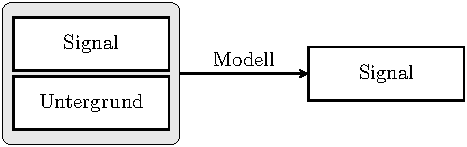
\includegraphics[scale=1]{./tikz/Target/Target.pdf}
	\end{figure}
  \end{block}
  \begin{block}{Simulierte Daten}<2>
	\begin{figure}
	  \centering
	  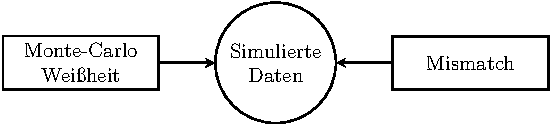
\includegraphics[scale=1]{./tikz/Mismatch/Mismatch.pdf}
	\end{figure}
  \end{block}
\end{frame}

\section{Modelle}
\begin{frame}{Entscheidungsbaum}
  \begin{columns}
	\column{.4\textwidth}
	\begin{figure}
	  \centering
	  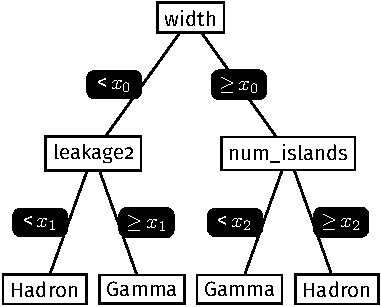
\includegraphics[width=\textwidth]{./tikz/Tree/Tree.pdf}
	\end{figure}
	\column{.6\textwidth}
	\begin{itemize}
	  \item Verknüpfte Abfragen 
	  \item Loss-function
	  \item Beschränkung der Komplexität 
	\end{itemize}
	\begin{table}	  
	  \centering
	  \begin{tabular}{c c c c c c}
		\toprule
		Ereignis & width & leakage2 & num\_islands & \dots & Konfi. \\ 
		\cmidrule(r){1-1} 	\cmidrule{2-5} \cmidrule(l){6-6}
		1 & \num{4.2}  & \num{0.4}  & \num{3} & \dots & \num{0.12} \\
		2 & \num{3.8}  & \num{0.0}  & \num{2} & \dots & \num{0.56} \\
		3 & \num{15.3} & \num{0.8} 	& \num{1} & \dots & \num{0.08} \\
		4 & \num{7.7}  & \num{0.1}  & \num{1} & \dots & \num{0.43} \\
		5 & \num{6.2}  & \num{0.0}  & \num{1} & \dots & \num{0.85} \\
		\bottomrule
	  \end{tabular}
	\end{table}
  \end{columns}
\end{frame}

\begin{frame}{Random Forest}
  \begin{columns}
	\column{.5\textwidth}
	\begin{figure}
	  \centering
	  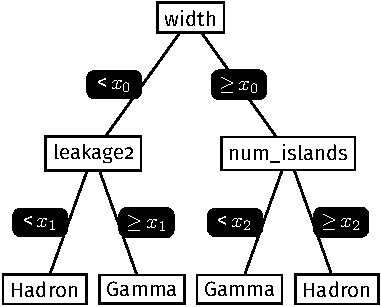
\includegraphics[scale=1]{./tikz/Tree/Tree.pdf}
	\end{figure}
	\column{.5\textwidth}
	\begin{figure}
	  \centering
	  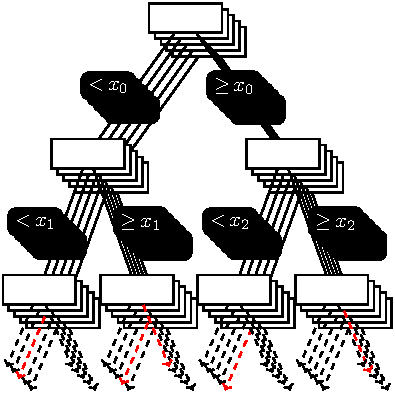
\includegraphics[scale=1]{./tikz/RandomForest/RandomForest.pdf}
	\end{figure}
  \end{columns}
\end{frame}

\begin{frame}{Random Forest}
  \begin{columns}
	\column{.4\textwidth}
	\begin{table}
	  \centering
	  \begin{tabular}{c c}
		\toprule
		Ereignis & Konfi. \\
		\cmidrule(r){1-1} \cmidrule(l){2-2}
		1 & \num{0.12} \\
		2 & \num{0.56} \\
		3 & \num{0.08} \\
		4 & \num{0.43} \\
		5 & \num{0.85} \\
		\bottomrule
	  \end{tabular}
	\end{table}
	\column{.6\textwidth}
	\begin{table}
	  \centering
	  \begin{tabular}{c c c c c c}
		\toprule
		Ereignis & Konf$_{1}$ & Konf$_{2}$ & Konf$_{3}$ & \dots & $\Sigma_\text{i}$ Konf$_\text{i}$ \\
		\cmidrule(r){1-1} \cmidrule(lr){2-5} \cmidrule(l){6-6}
		1 & \num{0.12} & \num{0.01} & \num{0.08} & \dots & \num{0.06} \\
		2 & \num{0.40} & \num{0.66} & \num{0.53} & \dots & \num{0.56} \\
		3 & \num{0.02} & \num{0.17} & \num{0.10} & \dots & \num{0.08} \\
		4 & \num{0.41} & \num{0.42} & \num{0.42} & \dots & \num{0.43} \\
		5 & \num{0.96} & \num{0.81} & \num{0.85} & \dots & \num{0.85} \\
		\bottomrule
	  \end{tabular}
	\end{table}
  \end{columns}
\end{frame}

\begin{frame}{Boosted Trees}
  \begin{columns}
	\column{.4\textwidth}
	\includegraphics<1>[width=\textwidth]{./tikz/BoostedTree/BoostedTree1.pdf}
	\includegraphics<2>[width=\textwidth]{./tikz/BoostedTree/BoostedTree2.pdf}
	\includegraphics<3>[width=\textwidth]{./tikz/BoostedTree/BoostedTree3.pdf}
	\includegraphics<4>[width=\textwidth]{./tikz/BoostedTree/BoostedTree.pdf}
	\column{.6\textwidth}
	\begin{itemize}
	  \item additives Training
	  \item höhere Gewichtung von Fehlklassifizierungen
	  \item ausgeglicherene Vorhersage
	  \item lässt sich nicht Parallelisieren
	  \item Modelle mit geringere Komplexität
	\end{itemize}
  \end{columns}
\end{frame}

\section{Ueberblick}
\begin{frame}
  \begin{figure}
	\centering
	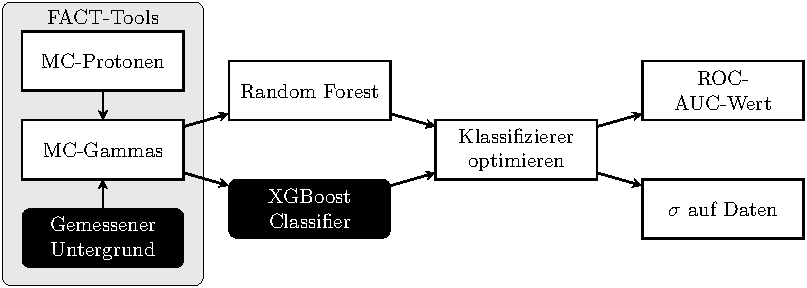
\includegraphics[width=\textwidth]{./tikz/Motiv/Motiv.pdf}
  \end{figure}
\end{frame}

\section{???}
\begin{frame}{Erstellen Trainingsdatensatzes}
  \begin{columns}
	\column{.5\textwidth}
	\begin{figure}
	  \centering
	  \includegraphics<1>[width=\textwidth]{./Plots/roc_info.pdf}
	  \includegraphics[width=\textwidth]<2>{./Plots/theta_cut.pdf}
	\end{figure}
	\column{.5\textwidth}
	Bereiningen der gemessen Daten von Gamma-Ereignissen 
	\begin{itemize}
	  \item ohne Eingang der Monte-Carlo Mismatche
	  \item moeglichst Reinen Datensatz
	  \item paar diffuse Gamma lassen sich physikalisch motivieren
	\end{itemize}
  \end{columns}
\end{frame}

\begin{frame}{Ueberpruefen Trainingsdatensatzes}
  \begin{columns}
	\column{.5\textwidth}
	\begin{figure}
	  \centering
	  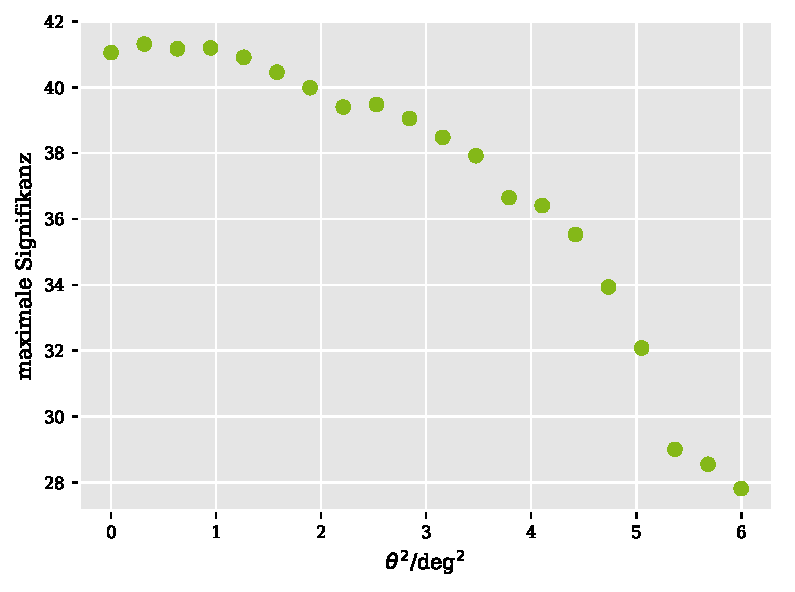
\includegraphics[width=\textwidth]{./Plots/corr_sig_theta2.pdf}
	\end{figure}
	\column{.5\textwidth}
	Trainingsdatensatz aus simulierte Gamma- und Proton-Ereignissen
	\begin{itemize}
	  \item Detektoreigenschaften fuer große $\theta$ signifikant
	  \item Signifikanz abhaengig vom $\theta$-Schnitt
	  \item \theta-Schnitt in Abhaengigkeit der Reinheit und korrelation der Signifikanz
	\end{itemize}
  \end{columns}
\end{frame}

\begin{frame}{Optimieren der Modelle}
  \begin{columns}
	\column{.5\textwidth}
	\begin{figure}
	  \centering
	  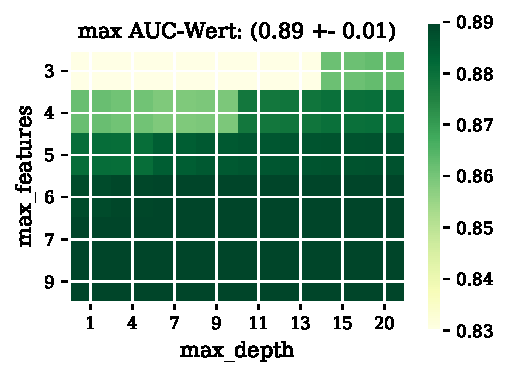
\includegraphics[scale=0.6]{./Plots/parameter_crab.pdf}
	\end{figure}
	\column{.5\textwidth}
	\begin{figure}
	  \centering
	  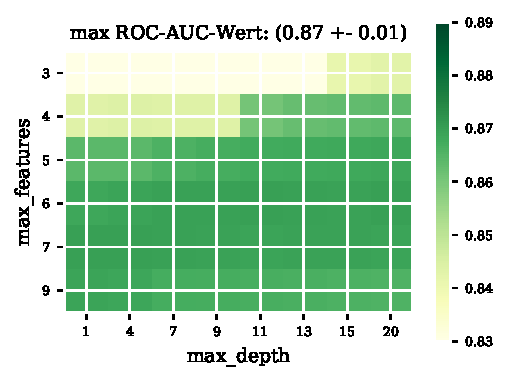
\includegraphics[scale=0.6]{./Plots/parameter_monte.pdf}
	\end{figure}
  \end{columns}
  \begin{table}[H]
	\centering
	\begin{tabular}{l s s}
	  \toprule
	  & MC-Daten & Messdaten \\
	  \cmidrule(r){2-3}
	  \texttt{XGBoost Classifier}	(Tiefe 1)	& \num{0.86(2)}	&\num{0.869(5)} \\ 
	  \texttt{Random Forrest}					& \num{0.87(1)} & \num{0.89(1)} \\
	  \bottomrule
	\end{tabular}
  \end{table}
\end{frame}

\section{Validieren auf echten Daten}

\begin{frame}
  \only<1-2>{
	\begin{figure}
	  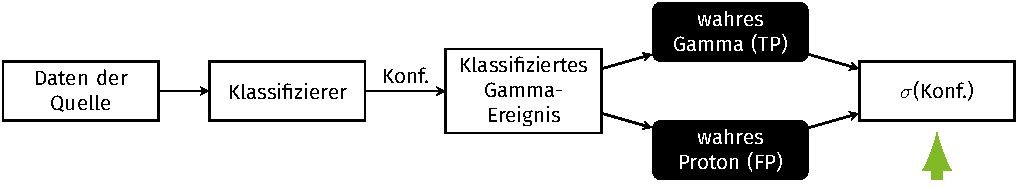
\includegraphics[width=\textwidth]{./tikz/Conf/Conf.pdf}
	\end{figure}
  }
  \only<2-2>{
	\begin{block}{Signifikanz}
	  \begin{equation*}
		S\left( N_\text{on}, N_\text{off}, S \right) = \sqrt{2} \left( N_\text{on} \ln \left[ \frac{1+ \alpha}{\alpha}\left( \frac{N_\text{on}}{N_\text{on} + N_\text{off}} \right) \right] + N_\text{off} \ln \left[ \left( 1+ \alpha \right) \left( \frac{N_\text{off}}{N_\text{on} + N_\text{off}} \right) \right] \right)^{1/2}
	  \end{equation*}
	\end{block}
  }
\end{frame}

\begin{frame}
  \only<1-2>{
	\begin{figure}
	  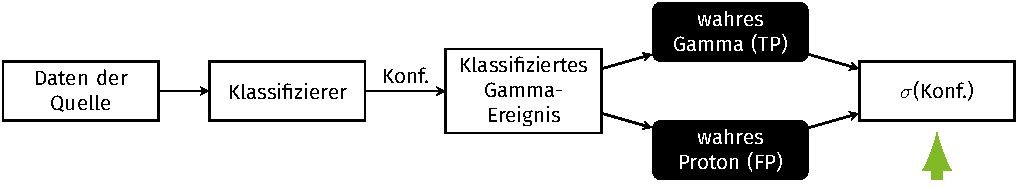
\includegraphics[width=0.5\textwidth]{./tikz/Conf/Conf.pdf}
	\end{figure}
  }
  \only<2-2>{
	\begin{figure}
	  \centering
	  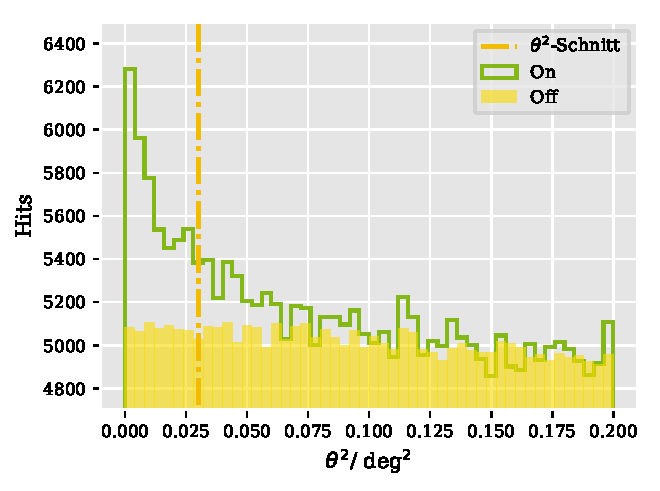
\includegraphics[height=0.7\textheight]{./Plots/on_off_ratio.pdf}
	\end{figure}
  }
\end{frame}

\begin{frame}
  \only<1-2>{
	\begin{figure}
	  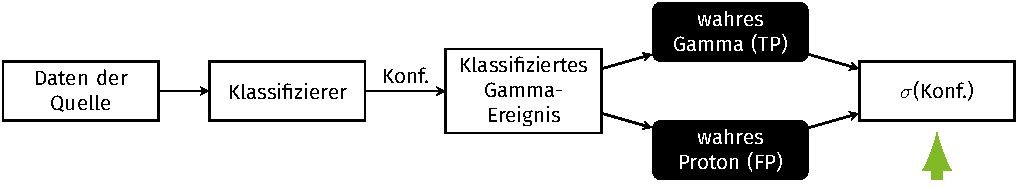
\includegraphics[width=0.5\textwidth]{./tikz/Conf/Conf.pdf}
	\end{figure}
  }
  \only<2-2>{
	\begin{columns}
	  \column{.5\textwidth}
	  \Large \bf Random Forest
	  \begin{itemize}
		\item komplexität
		\item viele Spezialisten auf ihrem Gebiet
		\item anfällig auf Training von Mismatche
	  \end{itemize}
	  \column{.5\textwidth}
	  \Large \bf XGBoost Classifier (Tiefe 1)
	  \begin{itemize}
		\item geringe Komplexität
		\item resistent gegen Mismatche
	  \end{itemize}
	\end{columns}
  }
\end{frame}

\begin{frame}
  \only<1-2>{
	\begin{figure}
	  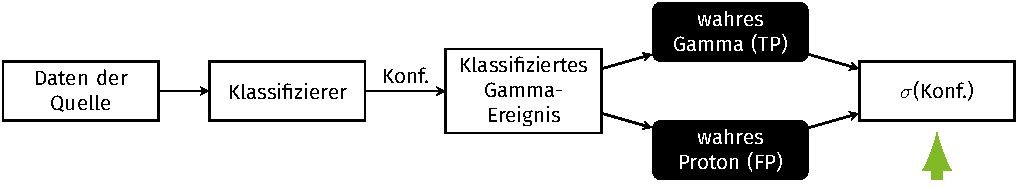
\includegraphics[width=0.5\textwidth]{./tikz/Conf/Conf.pdf}
	\end{figure}
  }
  \only<2-2>{
	\begin{figure}
	  \centering
	  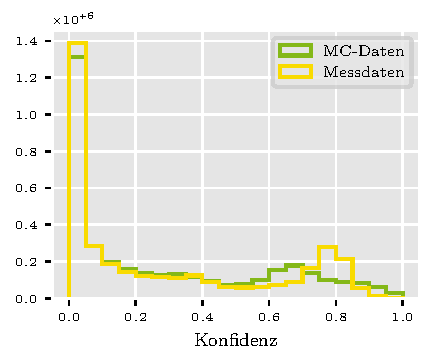
\includegraphics[width=0.5\textwidth]{Plots/conf.pdf}
	\end{figure}
  }
\end{frame}

\begin{frame}
  \only<1-2>{
	\begin{figure}
	  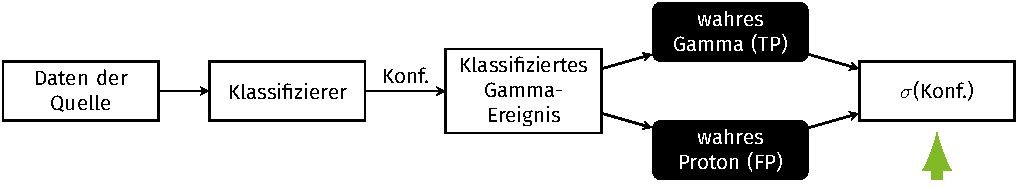
\includegraphics[width=0.5\textwidth]{./tikz/Conf/Conf.pdf}
	\end{figure}
  }
  \only<2-2>{
	\begin{figure}
	  \centering
	  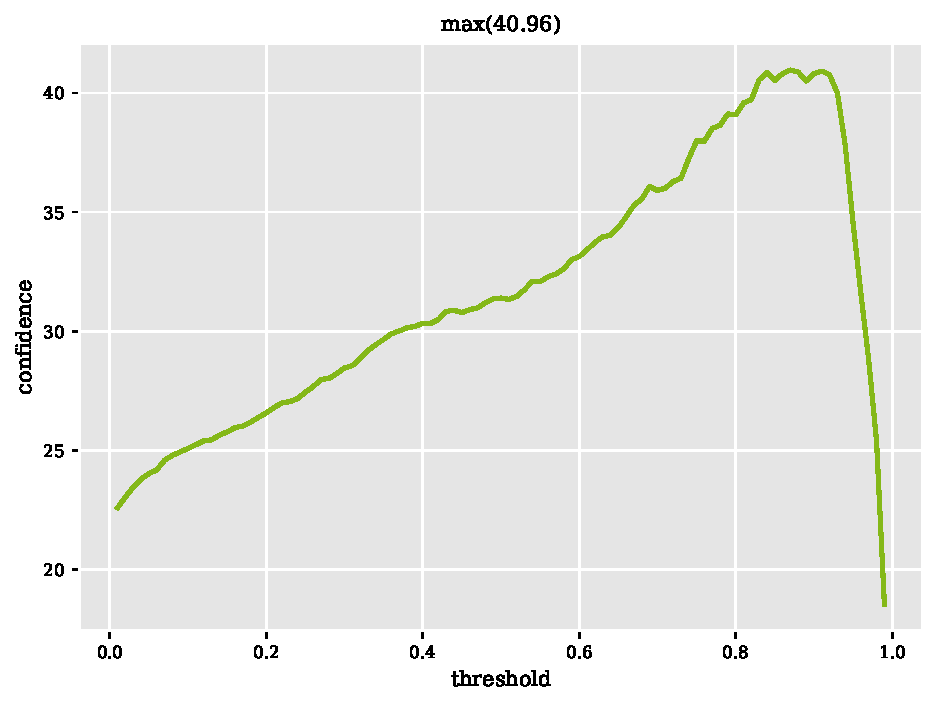
\includegraphics[height=0.8\textheight]{./Plots/significance_monte.pdf}
	\end{figure}
  }
\end{frame}

\begin{frame}
  \only<1-2>{
	\begin{figure}
	  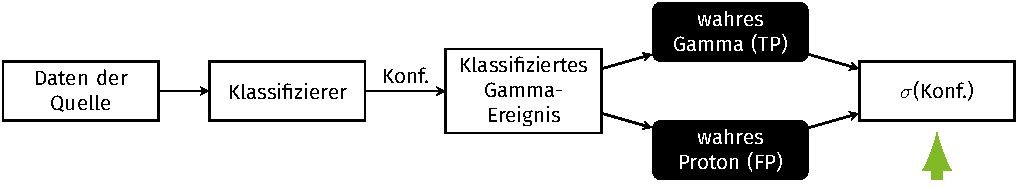
\includegraphics[width=0.5\textwidth]{./tikz/Conf/Conf.pdf}
	\end{figure}
  }
  \only<2-2>{
	\begin{table}
	  \begin{tabular}{l s s s s}
		\toprule 
		& \multicolumn{2}{c}{Krebsnebel}    & \multicolumn{2}{c}{Markarian 501} \\
		\cmidrule(r){2-3} \cmidrule(l){4-5}
		& Random & XGBoost        & Random & XGBoost   \\
		& Forest & (Tiefe= 1)   & Forest & (Tiefe= 1)\\
		unklassifizierte Daten & \multicolumn{2}{c}{\SI{21.4}{\sigma}}  & \multicolumn{2}{c}{\SI{17.1}{\sigma}} \\
		MC-Proton              & \SI{41.9}{\sigma}  & \SI{41.3}{\sigma} & \SI{35.5}{\sigma} & \SI{35.6}{\sigma}\\
		gemessene Proton       & \SI{32.9}{\sigma}  & \SI{37.8}{\sigma} & \SI{23.6}{\sigma} & \SI{35.2}{\sigma}\\
		\bottomrule
	  \end{tabular}
	\end{table}
  }
\end{frame}

\section{Mögliche Ursachen}

\begin{frame}{Thesen}
  \begin{itemize}
	\item<1-> Training auf Montecarlo Mismatches zur Seperation
	  \begin{itemize}
		\item komplexere Modelle weisen niedrigere Signifikanzen als einfachere Modelle auf.
	  \end{itemize}
	\item<2> Reduzierung schlecht simulierte Attribute
	  \begin{itemize}
		\item erhöhung der Signifikanz durch Reduzierung von Mismatches
	  \end{itemize}
  \end{itemize}
\end{frame}

\begin{frame}
  \Large \bf Achtung:
  \begin{itemize}
	\item Konfidenzverteilung nicht direkt vergleichbar
	\item Beide Bäume nach derselbem Kriterium gebaut
  \end{itemize}
  \begin{columns}
	\column{.5\textwidth}
	\Large \bf Random Forest
	\begin{figure}
	  \centering
	  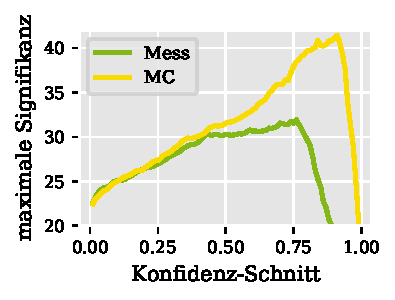
\includegraphics[width=0.8\textwidth]{./Plots/sig_mess_tree.pdf}
	\end{figure}
	\column{.5\textwidth}
	\Large \bf XGBoost Classifier (Tiefe 1)
	\begin{figure}
	  \centering
	  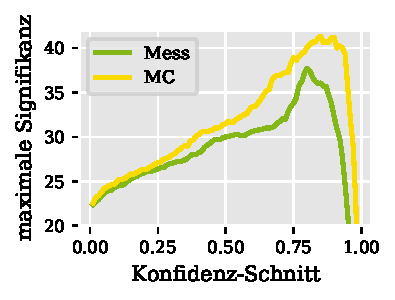
\includegraphics[width=0.8\textwidth]{./Plots/sig_mess_xgbc.pdf}
	\end{figure}
  \end{columns}
\end{frame}

\begin{frame}{Rekursive Feature Elimination}
  \begin{figure}
	\centering
	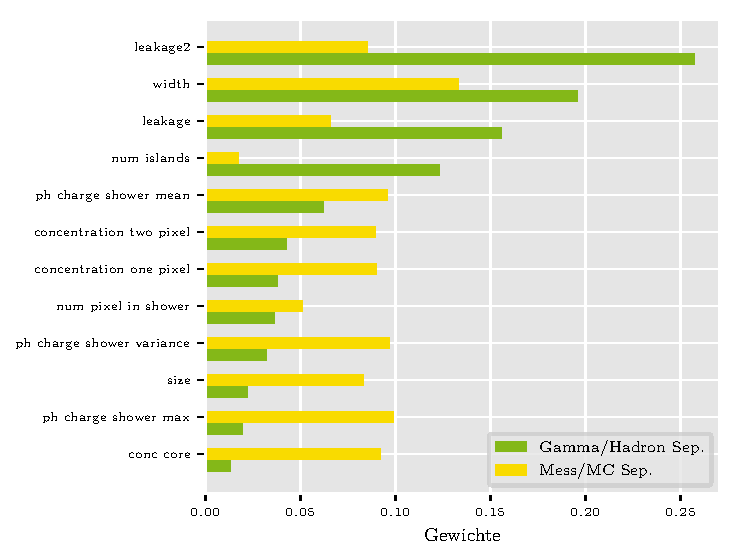
\includegraphics[height=0.8\textheight]{./Plots/feature_elemination.pdf}
  \end{figure}
\end{frame}

\begin{frame}
  \begin{table}
	\centering
	\begin{tabular}{l s s}
	  \toprule
	  & ohne Attribut & mit Attribut \\
	  & Eliminierung  & Eliminierung \\
	  \cmidrule(r){2-3}
	  ROC-AUC-Wert            & \num{0.64} & \num{0.61} \\
	  Li und Ma Signifikanz   & \SI{32.9}{\sigma} & \SI{34.4}{\sigma} \\
	  \bottomrule
	\end{tabular}
  \end{table}
\end{frame}

\section{Resüme}
\begin{frame}
  \begin{itemize}
	\item<1-> Unter den dieszeitigen Monte-Carlo-Simulationen wird die Simulation nicht verbessert 
	\item<2-> Verbesserung der Monte-Carlo-Simulationen 
	\item<3-> Datennahme von OFF-Daten
	\item<4-> Modell welches resistenter gegen Mismatches ist
  \end{itemize}
\end{frame}

\end{document}
